\documentclass[sigconf]{acmart}
\settopmatter{printacmref=false}
\usepackage{fancyvrb}
\usepackage{tabularx}
\usepackage{tikz}
\usepackage{hyperref}
%%
\makeatletter
\def\@copyrightspace{\relax}
\makeatother
%% \BibTeX command to typeset BibTeX logo in the docs
\begin{document}
\title{Dynamic Subdivision of Mass-Spring Cloth Simulations}
\author{Eleanor Olson}
\email{olsonk@rpi.edu}
\email{eleanorkolson@gmail.com}
\affiliation{
  \institution{Rensselaer Polytechnic Institute}
  \city{Troy}
  \state{New York}
  \country{USA}
}
\author{Kana Rudnick}
\email{rudnic2@rpi.edu}
\affiliation{
  \institution{Rensselaer Polytechnic Institute}
  \city{Troy}
  \state{New York}
  \country{USA}
}
\setcopyright{none}
\settopmatter{printacmref=false}
\renewcommand\footnotetextcopyrightpermission[1]{}
\pagestyle{plain}
 \citestyle{acmauthoryear}

\begin{abstract}
Representing cloth as a network of masses and springs is a common and effective method of simulating its behaviour. Traditionally, this network is uniformly dense across the surface; however, finding the ideal density for a given simulation can be challenging. This paper builds on previous work to automatically increase the density of mass-spring cloth simulations where necessary, simplifying the simulation process and increasing performance when compared with uniformly high-density simulations.
\end{abstract}

\keywords{Cloth animation, mass spring simulation, computer rendering}

\maketitle

\section{Introduction}
\subsection{Background}
The simulation of cloth is a deeply studied topic in computer graphics. With the frequency in which different
cloth-like structures are seen in animation, a need to develop a system that allows for a believable visualization
of the natural movement patterns of cloth is essential. Techniques like manual keyframe animation require too much effort
on the part of the animator, and doing such manual editing for all cloths found in the decorations and backgrounds of scenes
would take too much time. Therefore, attempts to simulate the physical behavior of cloth have been widely developed over time.

One of the most proficient methods for simulating cloth behavior has come from abstracting the cloth as a grid of
suspended masses connected using springs. This model allows for the simulation of real forces acting on these masses,
with the benefit of simplifying the representation to simple spring mass interactions. \cite{provot}

This method of simulation functions
well, but only if the given network of masses is sufficiently subdivided. This leads to an inevitable trade-off.

Too few masses will potentially lead to inaccurate simulation, especially around poles, corners, fixed points,
and other sensitive or complex regions in the mesh. Too many masses, in contrast, will lead to a more accurate simulation
at the cost of leading to a dramatic increase in the amount of computational effort needed to perform the simulation.

This paper proposes a method of simulation that finds a balance between computation time and accuracy. We propose a
system of dynamically subdividing the mesh during simulation time around complex regions while not subdividing other regions. This allows for an increase in the precision of the simulation at these complex regions while keeping
the overall granularity of the mesh, and therefore the computational time needed to simulate the movement of the mesh, low. 
\subsection{Preview}
We begin in section 2 with an overview of related work and methods that inspired our work. We then describe the details of our representation of the mesh, and how we subsequently simulate that representation in section 3. In section 4, we describe the algorithm for subdividing a portion of the mesh as well as the criteria used to determine when subdivision is necessary. Finally, we discuss the results of our method as well as future work and improvements that can be made.
\section{Related Work}
\subsection{Mass Spring Cloth Simulation}
One of the largest sources of inspiration for this work is that of Provot \cite{provot}. He defines the system of mass-spring discretizations that we use as the basis for our representation of the mesh during simulation. This mass-spring representation allows for the simulation to only be dependent on simulating the motion of and forces acting on every particle independently, rather than having to accurately model the entire cloth as a whole. The paper also describes a simple yet effective system for managing inaccurate "super-elastic" deformations in the simulation, allowing for a successfully convincing simulation without requiring significant computational costs. Provot's methods work very well for most basic applications, and are rather simple to implement. 

Due to this simplicity, there are aspects of the method that can be improved. For a grid of n particles along the x-axis and m particles along the y-axis, a subdivision that transforms every quad in the mesh into four quads results in a grid of particles $2n$ by $2m$. This means that using Provot's method, a single level of subdivision results in four times as many particles that must be simulated at every timestep: a dramatic increase in computational time. 
\subsection{Subdividing Cloth Simulation}
Previous work has been done in running cloth simulations with dynamic subdivision. One such work that served as the primary inspiration for our work is that of Hutchinson, Preston, and Hewitt \cite{hutchinson}. The authors propose a method for simulating a cloth that has varying levels of subdivision throughout the mesh.
This is accomplished through the use of a data structure that represents the full network, with each mass keeping track of what level of subdivision the mass is located on. They also propose a simple method of using the angle between neighboring masses to determine whether a point must undergo subdivision before simulation can be performed.

The technique, while simple, is effective in most cases. However, it lacks in a few areas, most notably in that due to the subdivision detection algorithm relying on neighboring masses, it fails to be effective at detecting if points that lack enough neighbors, including points on edges or points within a mesh that has not been subdivided at all in a given region. We look to improve upon this in our implementation, allowing for a thorough detection of when subdivision is necessary in all situations.
\section{Method of Simulation}
\subsection{Representing Cloth in Data}
The underlying model of our simulation is directly built on the work described in \cite{hutchinson}. We construct a 2 dimensional grid of indices, each containing one of the following types of mass particles:
\begin{itemize}
\item Active: A particle that is actively simulated and may move freely
\item Fixed: A particle that exists and contributes spring forces to adjacent particles, however may not itself move in space.
\item Interpolated: A particle that is not actively simulated, and instead interpolates its position between neighboring particles. These particles also contribute spring forces to adjacent particles.
\item None: No particle exists at this index. This occurs when one section of the cloth is subdivided, and therefore requires other sections to have "gaps" in the underlying representation.
\end{itemize} 
All of these particles, excluding "None" particles, contain their current position and velocity, as well as their subdivision "layer". Particles created at the beginning of simulation begin on layer 0, and any subdivision increases a particle's layer by 1, as well as creating particles of that same higher layer around it.
\subsection{Theory of Simulation}
As in \cite{hutchinson}, we begin with an input cloth of uniform, ideally low, mass density. To simulate this mesh without any subdivision, we follow a process identical to that laid out in \cite{provot}. This entails iterating over each particle in the mesh and calculating the forces on it by adjacent springs, as well as any outside forces such as gravity. These forces are then integrated via explicit Euler integration, updating each particle's velocity, which is in turn explicitly integrated to update the particle's position. 

To simulate a mesh with arbitrary subdivision, we follow a similar approach. We once again iterate over all possible indices in the graph, however not all indices will have existing particles. Therefore, we ignore all particles of type "None". Additionally, since the force on any given "Fixed" or "Interpolated" particle will not affect its position, these too may be skipped over. 

To calculate the forces affecting a particle, we must find all springs connected to it. There are 3 different forms of springs in our simulation:
\begin{itemize}
\item Structural: Directly adjacent in 1 axis ($x\pm$1 or $y\pm1$)
\item Shear: Adjacent along the diagonal ($x,y\pm1$)
\item Bend:  1 particle away in 1 axis($x\pm2$ or $y\pm 2$)
\end{itemize}
These spring types can also be seen in Figure \ref{fig:springs}.
\begin{figure}


\tikzset{every picture/.style={line width=0.75pt}} %set default line width to 0.75pt        

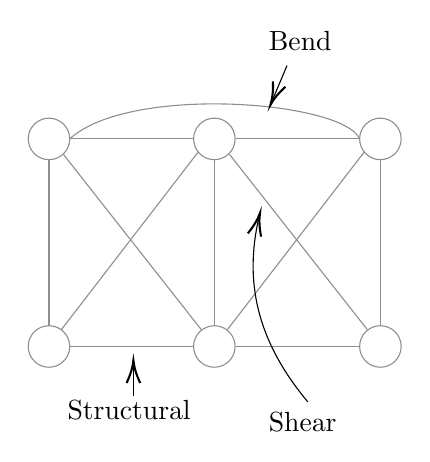
\begin{tikzpicture}[x=0.75pt,y=0.75pt,yscale=-1,xscale=1]
%uncomment if require: \path (0,300); %set diagram left start at 0, and has height of 300

%Shape: Circle [id:dp7708110690404341] 
\draw  [color={rgb, 255:red, 144; green, 141; blue, 141 }  ,draw opacity=1 ] (61.33,82.33) .. controls (61.33,76.81) and (65.81,72.33) .. (71.33,72.33) .. controls (76.86,72.33) and (81.33,76.81) .. (81.33,82.33) .. controls (81.33,87.86) and (76.86,92.33) .. (71.33,92.33) .. controls (65.81,92.33) and (61.33,87.86) .. (61.33,82.33) -- cycle ;
%Shape: Circle [id:dp7665280557032523] 
\draw  [color={rgb, 255:red, 144; green, 141; blue, 141 }  ,draw opacity=1 ] (141,82.33) .. controls (141,76.81) and (145.48,72.33) .. (151,72.33) .. controls (156.52,72.33) and (161,76.81) .. (161,82.33) .. controls (161,87.86) and (156.52,92.33) .. (151,92.33) .. controls (145.48,92.33) and (141,87.86) .. (141,82.33) -- cycle ;
%Shape: Circle [id:dp8143191905899676] 
\draw  [color={rgb, 255:red, 144; green, 141; blue, 141 }  ,draw opacity=1 ] (61.33,182.33) .. controls (61.33,176.81) and (65.81,172.33) .. (71.33,172.33) .. controls (76.86,172.33) and (81.33,176.81) .. (81.33,182.33) .. controls (81.33,187.86) and (76.86,192.33) .. (71.33,192.33) .. controls (65.81,192.33) and (61.33,187.86) .. (61.33,182.33) -- cycle ;
%Shape: Circle [id:dp055131028649787805] 
\draw  [color={rgb, 255:red, 144; green, 141; blue, 141 }  ,draw opacity=1 ] (141,182.33) .. controls (141,176.81) and (145.48,172.33) .. (151,172.33) .. controls (156.52,172.33) and (161,176.81) .. (161,182.33) .. controls (161,187.86) and (156.52,192.33) .. (151,192.33) .. controls (145.48,192.33) and (141,187.86) .. (141,182.33) -- cycle ;
%Straight Lines [id:da4031336052941048] 
\draw [color={rgb, 255:red, 144; green, 141; blue, 141 }  ,draw opacity=1 ]   (81.33,82.33) -- (141,82.33) ;
%Straight Lines [id:da8685025102332997] 
\draw [color={rgb, 255:red, 144; green, 141; blue, 141 }  ,draw opacity=1 ]   (151,172.33) -- (151,92.33) ;
%Straight Lines [id:da6758735308566833] 
\draw [color={rgb, 255:red, 144; green, 141; blue, 141 }  ,draw opacity=1 ]   (141,182.33) -- (81.33,182.33) ;
%Straight Lines [id:da8974623371735779] 
\draw [color={rgb, 255:red, 144; green, 141; blue, 141 }  ,draw opacity=1 ]   (71.33,92.33) -- (71.33,172.33) ;
%Straight Lines [id:da6410792423648672] 
\draw [color={rgb, 255:red, 144; green, 141; blue, 141 }  ,draw opacity=1 ]   (78.33,89.83) -- (144.67,174.17) ;
%Straight Lines [id:da5559775946796298] 
\draw [color={rgb, 255:red, 144; green, 141; blue, 141 }  ,draw opacity=1 ]   (143.33,88.5) -- (77.33,174.17) ;
%Shape: Circle [id:dp4432221630176525] 
\draw  [color={rgb, 255:red, 144; green, 141; blue, 141 }  ,draw opacity=1 ] (221,82.33) .. controls (221,76.81) and (225.48,72.33) .. (231,72.33) .. controls (236.52,72.33) and (241,76.81) .. (241,82.33) .. controls (241,87.86) and (236.52,92.33) .. (231,92.33) .. controls (225.48,92.33) and (221,87.86) .. (221,82.33) -- cycle ;
%Shape: Circle [id:dp24251645493662155] 
\draw  [color={rgb, 255:red, 144; green, 141; blue, 141 }  ,draw opacity=1 ] (221,182.33) .. controls (221,176.81) and (225.48,172.33) .. (231,172.33) .. controls (236.52,172.33) and (241,176.81) .. (241,182.33) .. controls (241,187.86) and (236.52,192.33) .. (231,192.33) .. controls (225.48,192.33) and (221,187.86) .. (221,182.33) -- cycle ;
%Straight Lines [id:da49718671637024137] 
\draw [color={rgb, 255:red, 144; green, 141; blue, 141 }  ,draw opacity=1 ]   (161.33,82.33) -- (221,82.33) ;
%Straight Lines [id:da09899274633352273] 
\draw [color={rgb, 255:red, 144; green, 141; blue, 141 }  ,draw opacity=1 ]   (231,172.33) -- (231,92.33) ;
%Straight Lines [id:da966939397900791] 
\draw [color={rgb, 255:red, 144; green, 141; blue, 141 }  ,draw opacity=1 ]   (221,182.33) -- (161.33,182.33) ;
%Straight Lines [id:da32590548525237795] 
\draw [color={rgb, 255:red, 144; green, 141; blue, 141 }  ,draw opacity=1 ]   (158.33,89.83) -- (224.67,174.17) ;
%Straight Lines [id:da7236689415661267] 
\draw [color={rgb, 255:red, 144; green, 141; blue, 141 }  ,draw opacity=1 ]   (223.33,88.5) -- (157.33,174.17) ;
%Straight Lines [id:da8340397740061083] 
\draw    (112,206) -- (112,191) ;
\draw [shift={(112,189)}, rotate = 90] [color={rgb, 255:red, 0; green, 0; blue, 0 }  ][line width=0.75]    (10.93,-3.29) .. controls (6.95,-1.4) and (3.31,-0.3) .. (0,0) .. controls (3.31,0.3) and (6.95,1.4) .. (10.93,3.29)   ;
%Curve Lines [id:da6718169798399151] 
\draw    (196,209) .. controls (171.5,179.6) and (165.25,151.16) .. (172.54,119.92) ;
\draw [shift={(173,118)}, rotate = 104.04] [color={rgb, 255:red, 0; green, 0; blue, 0 }  ][line width=0.75]    (10.93,-3.29) .. controls (6.95,-1.4) and (3.31,-0.3) .. (0,0) .. controls (3.31,0.3) and (6.95,1.4) .. (10.93,3.29)   ;
%Curve Lines [id:da7096064606011079] 
\draw [color={rgb, 255:red, 144; green, 141; blue, 141 }  ,draw opacity=1 ]   (81.33,82.33) .. controls (110,56) and (213,64) .. (221,82.33) ;
%Straight Lines [id:da28289438666079003] 
\draw    (186,47) -- (178.78,64.16) ;
\draw [shift={(178,66)}, rotate = 292.83] [color={rgb, 255:red, 0; green, 0; blue, 0 }  ][line width=0.75]    (10.93,-3.29) .. controls (6.95,-1.4) and (3.31,-0.3) .. (0,0) .. controls (3.31,0.3) and (6.95,1.4) .. (10.93,3.29)   ;

% Text Node
\draw (79,207) node [anchor=north west][inner sep=0.75pt]   [align=left] {Structural};
% Text Node
\draw (176,29) node [anchor=north west][inner sep=0.75pt]   [align=left] {Bend};
% Text Node
\draw (176,213) node [anchor=north west][inner sep=0.75pt]   [align=left] {Shear};


\end{tikzpicture}
\caption{Example of different types of springs in the simulation.}
\label{fig:springs}
\end{figure}

The distance between springs, however, must be scaled depending on the layer $l$ of the particle. Given a particle at layer 0, if the underlying mesh can represent 1 extra subdivision we know that we must skip over 1 index to get to the next particle of layer 0. This can be generalized for all layers as the following: if we take $m$ as the maximum subdivision our underlying data structure can represent, we know that a particle on the same layer $l$ will be $2^{m-l}$ indices offset. Therefore, we scale all spring distances by this factor.

In addition to properly finding adjacent springs in the mesh, the key insight from \cite{hutchinson} to simulate areas of differing subdivision smoothly is to simulate them multiple times per animation step. We recalculate forces, velocities, and positions for each particle $2^{l}$ times, where $l$ is the particle's layer. Finally, we adjust particle positions to be maximally extended by an input parameter, avoiding hyperextended springs using the techniques from \cite{provot}. Overall, this simulation takes the form shown in Figure \ref{fig:sim}.
\begin{figure}
\begin{Verbatim}
x, y = dimension of cloth
m = maximum subdivision layer in cloth
for t in 0..2^m, i in 0..x, j in 0..y:
	p = particle(i,j)
	if p.type != Active:
            continue
        if p.layer < t:
		forces = forces(p)
		p.velocity += forces*timestep
		p.position += velocity*timestep
		p.position = correct(p.position)

\end{Verbatim}
\caption{Pseudocode of Cloth Simulation}
\label{fig:sim}
\end{figure}

\subsection{Rendering}
In traditional, uniform mass-spring simulation, it is trivial to construct a quad by connecting to the points directly adjacent. This step is required to pass our cloth into a rendering pipeline and display it to the screen. In a subdivided cloth, however, this step becomes nontrivial.

To generate these quads, we begin by iterating over our mesh. When we find a particle that is not of type "None", we know that this will be the corner of one of our mesh's quads. Further, due to our subdivision scheme, discussed further in Section 4.1, we know that our cloth mesh will always decompose into square quads of the underlying mesh. That is to say, that each quad will have particles at indices $(i,j), (i+k, j), (i,j+k), (i+k,j+k)$, where $(i,j)$ is our initial point, and $k$ is some constant. To find this $k$, we check each index in the cloth mesh $(i+k,j+k), 0\leq k$, until we find a particle not of type "None". We then pass all four of these particles' positions into the renderer. Finally, we skip our iteration to next check point $(i,j+k)$, the particle ending the quad on our iterated row.

While this method of quad generation works in most cases, it has the potential to create extraneous quads in the mesh. One situation where this occurs is shown in Figure \ref{fig:interp}, which finds a corner to construct but should not actually create a new quad. Due to the guarantee of square output quad generation, these artifacts can only appear when extending a diagonal from an "Interpolated" particle. Therefore, we assign each interpolated particle a layer $l$ corresponding to the subdivision layer that generates it. We then bound the maximum value of $k \leq 2^{m-l}$, where $m$ is the maximum subdivision represented in the cloth mesh. If no particle is found within $0\leq k \leq 2^{m-l}$, the particle is skipped over. This technique allows us to robustly convert our subdivided cloth mesh into a series of quads that can be easily rendered.

\begin{figure}


\tikzset{every picture/.style={line width=0.75pt}} %set default line width to 0.75pt        

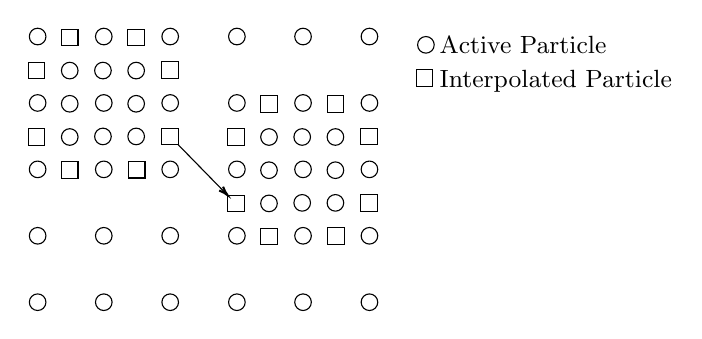
\begin{tikzpicture}[x=0.3pt,y=0.3pt,yscale=-1,xscale=1]
%uncomment if require: \path (0,425); %set diagram left start at 0, and has height of 425

%Shape: Circle [id:dp28714526119034034] 
\draw   (30.33,30.33) .. controls (30.33,24.81) and (34.81,20.33) .. (40.33,20.33) .. controls (45.86,20.33) and (50.33,24.81) .. (50.33,30.33) .. controls (50.33,35.86) and (45.86,40.33) .. (40.33,40.33) .. controls (34.81,40.33) and (30.33,35.86) .. (30.33,30.33) -- cycle ;
%Shape: Circle [id:dp9405531663649225] 
\draw   (110,30.33) .. controls (110,24.81) and (114.48,20.33) .. (120,20.33) .. controls (125.52,20.33) and (130,24.81) .. (130,30.33) .. controls (130,35.86) and (125.52,40.33) .. (120,40.33) .. controls (114.48,40.33) and (110,35.86) .. (110,30.33) -- cycle ;
%Shape: Circle [id:dp000891091912133879] 
\draw   (190,30.33) .. controls (190,24.81) and (194.48,20.33) .. (200,20.33) .. controls (205.52,20.33) and (210,24.81) .. (210,30.33) .. controls (210,35.86) and (205.52,40.33) .. (200,40.33) .. controls (194.48,40.33) and (190,35.86) .. (190,30.33) -- cycle ;
%Shape: Circle [id:dp2654804735412266] 
\draw   (30.33,110.33) .. controls (30.33,104.81) and (34.81,100.33) .. (40.33,100.33) .. controls (45.86,100.33) and (50.33,104.81) .. (50.33,110.33) .. controls (50.33,115.86) and (45.86,120.33) .. (40.33,120.33) .. controls (34.81,120.33) and (30.33,115.86) .. (30.33,110.33) -- cycle ;
%Shape: Circle [id:dp42179985152857613] 
\draw   (110,110.33) .. controls (110,104.81) and (114.48,100.33) .. (120,100.33) .. controls (125.52,100.33) and (130,104.81) .. (130,110.33) .. controls (130,115.86) and (125.52,120.33) .. (120,120.33) .. controls (114.48,120.33) and (110,115.86) .. (110,110.33) -- cycle ;
%Shape: Circle [id:dp22630394337930826] 
\draw   (190,110.33) .. controls (190,104.81) and (194.48,100.33) .. (200,100.33) .. controls (205.52,100.33) and (210,104.81) .. (210,110.33) .. controls (210,115.86) and (205.52,120.33) .. (200,120.33) .. controls (194.48,120.33) and (190,115.86) .. (190,110.33) -- cycle ;
%Shape: Circle [id:dp6688016654819198] 
\draw   (30.33,190.33) .. controls (30.33,184.81) and (34.81,180.33) .. (40.33,180.33) .. controls (45.86,180.33) and (50.33,184.81) .. (50.33,190.33) .. controls (50.33,195.86) and (45.86,200.33) .. (40.33,200.33) .. controls (34.81,200.33) and (30.33,195.86) .. (30.33,190.33) -- cycle ;
%Shape: Circle [id:dp7311547975312614] 
\draw   (110,190.33) .. controls (110,184.81) and (114.48,180.33) .. (120,180.33) .. controls (125.52,180.33) and (130,184.81) .. (130,190.33) .. controls (130,195.86) and (125.52,200.33) .. (120,200.33) .. controls (114.48,200.33) and (110,195.86) .. (110,190.33) -- cycle ;
%Shape: Circle [id:dp9364435671025728] 
\draw   (190,190.33) .. controls (190,184.81) and (194.48,180.33) .. (200,180.33) .. controls (205.52,180.33) and (210,184.81) .. (210,190.33) .. controls (210,195.86) and (205.52,200.33) .. (200,200.33) .. controls (194.48,200.33) and (190,195.86) .. (190,190.33) -- cycle ;
%Shape: Circle [id:dp30541198839696815] 
\draw   (270.33,30.33) .. controls (270.33,24.81) and (274.81,20.33) .. (280.33,20.33) .. controls (285.86,20.33) and (290.33,24.81) .. (290.33,30.33) .. controls (290.33,35.86) and (285.86,40.33) .. (280.33,40.33) .. controls (274.81,40.33) and (270.33,35.86) .. (270.33,30.33) -- cycle ;
%Shape: Circle [id:dp9946449484262146] 
\draw   (350,30.33) .. controls (350,24.81) and (354.48,20.33) .. (360,20.33) .. controls (365.52,20.33) and (370,24.81) .. (370,30.33) .. controls (370,35.86) and (365.52,40.33) .. (360,40.33) .. controls (354.48,40.33) and (350,35.86) .. (350,30.33) -- cycle ;
%Shape: Circle [id:dp43180225697273056] 
\draw   (430,30.33) .. controls (430,24.81) and (434.48,20.33) .. (440,20.33) .. controls (445.52,20.33) and (450,24.81) .. (450,30.33) .. controls (450,35.86) and (445.52,40.33) .. (440,40.33) .. controls (434.48,40.33) and (430,35.86) .. (430,30.33) -- cycle ;
%Shape: Circle [id:dp3880344571042218] 
\draw   (270.33,110.33) .. controls (270.33,104.81) and (274.81,100.33) .. (280.33,100.33) .. controls (285.86,100.33) and (290.33,104.81) .. (290.33,110.33) .. controls (290.33,115.86) and (285.86,120.33) .. (280.33,120.33) .. controls (274.81,120.33) and (270.33,115.86) .. (270.33,110.33) -- cycle ;
%Shape: Circle [id:dp94187688676629] 
\draw   (350,110.33) .. controls (350,104.81) and (354.48,100.33) .. (360,100.33) .. controls (365.52,100.33) and (370,104.81) .. (370,110.33) .. controls (370,115.86) and (365.52,120.33) .. (360,120.33) .. controls (354.48,120.33) and (350,115.86) .. (350,110.33) -- cycle ;
%Shape: Circle [id:dp5700440423803386] 
\draw   (430,110.33) .. controls (430,104.81) and (434.48,100.33) .. (440,100.33) .. controls (445.52,100.33) and (450,104.81) .. (450,110.33) .. controls (450,115.86) and (445.52,120.33) .. (440,120.33) .. controls (434.48,120.33) and (430,115.86) .. (430,110.33) -- cycle ;
%Shape: Circle [id:dp27226414031535673] 
\draw   (270.33,190.33) .. controls (270.33,184.81) and (274.81,180.33) .. (280.33,180.33) .. controls (285.86,180.33) and (290.33,184.81) .. (290.33,190.33) .. controls (290.33,195.86) and (285.86,200.33) .. (280.33,200.33) .. controls (274.81,200.33) and (270.33,195.86) .. (270.33,190.33) -- cycle ;
%Shape: Circle [id:dp47075637284141547] 
\draw   (350,190.33) .. controls (350,184.81) and (354.48,180.33) .. (360,180.33) .. controls (365.52,180.33) and (370,184.81) .. (370,190.33) .. controls (370,195.86) and (365.52,200.33) .. (360,200.33) .. controls (354.48,200.33) and (350,195.86) .. (350,190.33) -- cycle ;
%Shape: Circle [id:dp9031450571582846] 
\draw   (430,190.33) .. controls (430,184.81) and (434.48,180.33) .. (440,180.33) .. controls (445.52,180.33) and (450,184.81) .. (450,190.33) .. controls (450,195.86) and (445.52,200.33) .. (440,200.33) .. controls (434.48,200.33) and (430,195.86) .. (430,190.33) -- cycle ;
%Shape: Circle [id:dp02413050267565342] 
\draw   (30.33,270.33) .. controls (30.33,264.81) and (34.81,260.33) .. (40.33,260.33) .. controls (45.86,260.33) and (50.33,264.81) .. (50.33,270.33) .. controls (50.33,275.86) and (45.86,280.33) .. (40.33,280.33) .. controls (34.81,280.33) and (30.33,275.86) .. (30.33,270.33) -- cycle ;
%Shape: Circle [id:dp38230282023508355] 
\draw   (110,270.33) .. controls (110,264.81) and (114.48,260.33) .. (120,260.33) .. controls (125.52,260.33) and (130,264.81) .. (130,270.33) .. controls (130,275.86) and (125.52,280.33) .. (120,280.33) .. controls (114.48,280.33) and (110,275.86) .. (110,270.33) -- cycle ;
%Shape: Circle [id:dp315220024090222] 
\draw   (190,270.33) .. controls (190,264.81) and (194.48,260.33) .. (200,260.33) .. controls (205.52,260.33) and (210,264.81) .. (210,270.33) .. controls (210,275.86) and (205.52,280.33) .. (200,280.33) .. controls (194.48,280.33) and (190,275.86) .. (190,270.33) -- cycle ;
%Shape: Circle [id:dp6847420475233083] 
\draw   (30.33,350.33) .. controls (30.33,344.81) and (34.81,340.33) .. (40.33,340.33) .. controls (45.86,340.33) and (50.33,344.81) .. (50.33,350.33) .. controls (50.33,355.86) and (45.86,360.33) .. (40.33,360.33) .. controls (34.81,360.33) and (30.33,355.86) .. (30.33,350.33) -- cycle ;
%Shape: Circle [id:dp46430522629414084] 
\draw   (110,350.33) .. controls (110,344.81) and (114.48,340.33) .. (120,340.33) .. controls (125.52,340.33) and (130,344.81) .. (130,350.33) .. controls (130,355.86) and (125.52,360.33) .. (120,360.33) .. controls (114.48,360.33) and (110,355.86) .. (110,350.33) -- cycle ;
%Shape: Circle [id:dp7179447926403252] 
\draw   (190,350.33) .. controls (190,344.81) and (194.48,340.33) .. (200,340.33) .. controls (205.52,340.33) and (210,344.81) .. (210,350.33) .. controls (210,355.86) and (205.52,360.33) .. (200,360.33) .. controls (194.48,360.33) and (190,355.86) .. (190,350.33) -- cycle ;
%Shape: Circle [id:dp014683573380622317] 
\draw   (270.33,270.33) .. controls (270.33,264.81) and (274.81,260.33) .. (280.33,260.33) .. controls (285.86,260.33) and (290.33,264.81) .. (290.33,270.33) .. controls (290.33,275.86) and (285.86,280.33) .. (280.33,280.33) .. controls (274.81,280.33) and (270.33,275.86) .. (270.33,270.33) -- cycle ;
%Shape: Circle [id:dp4103461557658463] 
\draw   (350,270.33) .. controls (350,264.81) and (354.48,260.33) .. (360,260.33) .. controls (365.52,260.33) and (370,264.81) .. (370,270.33) .. controls (370,275.86) and (365.52,280.33) .. (360,280.33) .. controls (354.48,280.33) and (350,275.86) .. (350,270.33) -- cycle ;
%Shape: Circle [id:dp15827515828040772] 
\draw   (430,270.33) .. controls (430,264.81) and (434.48,260.33) .. (440,260.33) .. controls (445.52,260.33) and (450,264.81) .. (450,270.33) .. controls (450,275.86) and (445.52,280.33) .. (440,280.33) .. controls (434.48,280.33) and (430,275.86) .. (430,270.33) -- cycle ;
%Shape: Circle [id:dp6297916028178151] 
\draw   (270.33,350.33) .. controls (270.33,344.81) and (274.81,340.33) .. (280.33,340.33) .. controls (285.86,340.33) and (290.33,344.81) .. (290.33,350.33) .. controls (290.33,355.86) and (285.86,360.33) .. (280.33,360.33) .. controls (274.81,360.33) and (270.33,355.86) .. (270.33,350.33) -- cycle ;
%Shape: Circle [id:dp812817138463636] 
\draw   (350,350.33) .. controls (350,344.81) and (354.48,340.33) .. (360,340.33) .. controls (365.52,340.33) and (370,344.81) .. (370,350.33) .. controls (370,355.86) and (365.52,360.33) .. (360,360.33) .. controls (354.48,360.33) and (350,355.86) .. (350,350.33) -- cycle ;
%Shape: Circle [id:dp4606860898228706] 
\draw   (430,350.33) .. controls (430,344.81) and (434.48,340.33) .. (440,340.33) .. controls (445.52,340.33) and (450,344.81) .. (450,350.33) .. controls (450,355.86) and (445.52,360.33) .. (440,360.33) .. controls (434.48,360.33) and (430,355.86) .. (430,350.33) -- cycle ;
%Shape: Circle [id:dp43593890291085824] 
\draw   (109,71.33) .. controls (109,65.81) and (113.48,61.33) .. (119,61.33) .. controls (124.52,61.33) and (129,65.81) .. (129,71.33) .. controls (129,76.86) and (124.52,81.33) .. (119,81.33) .. controls (113.48,81.33) and (109,76.86) .. (109,71.33) -- cycle ;
%Shape: Circle [id:dp9630078831488638] 
\draw   (149,71.33) .. controls (149,65.81) and (153.48,61.33) .. (159,61.33) .. controls (164.52,61.33) and (169,65.81) .. (169,71.33) .. controls (169,76.86) and (164.52,81.33) .. (159,81.33) .. controls (153.48,81.33) and (149,76.86) .. (149,71.33) -- cycle ;
%Shape: Circle [id:dp0629356162786795] 
\draw   (149,111.33) .. controls (149,105.81) and (153.48,101.33) .. (159,101.33) .. controls (164.52,101.33) and (169,105.81) .. (169,111.33) .. controls (169,116.86) and (164.52,121.33) .. (159,121.33) .. controls (153.48,121.33) and (149,116.86) .. (149,111.33) -- cycle ;
%Shape: Circle [id:dp48729488805580634] 
\draw   (149,150.67) .. controls (149,145.14) and (153.48,140.67) .. (159,140.67) .. controls (164.52,140.67) and (169,145.14) .. (169,150.67) .. controls (169,156.19) and (164.52,160.67) .. (159,160.67) .. controls (153.48,160.67) and (149,156.19) .. (149,150.67) -- cycle ;
%Shape: Circle [id:dp2269764043911061] 
\draw   (109,150.67) .. controls (109,145.14) and (113.48,140.67) .. (119,140.67) .. controls (124.52,140.67) and (129,145.14) .. (129,150.67) .. controls (129,156.19) and (124.52,160.67) .. (119,160.67) .. controls (113.48,160.67) and (109,156.19) .. (109,150.67) -- cycle ;
%Shape: Circle [id:dp6211820650136616] 
\draw   (69,151.33) .. controls (69,145.81) and (73.48,141.33) .. (79,141.33) .. controls (84.52,141.33) and (89,145.81) .. (89,151.33) .. controls (89,156.86) and (84.52,161.33) .. (79,161.33) .. controls (73.48,161.33) and (69,156.86) .. (69,151.33) -- cycle ;
%Shape: Circle [id:dp15071324664817887] 
\draw   (69,111.33) .. controls (69,105.81) and (73.48,101.33) .. (79,101.33) .. controls (84.52,101.33) and (89,105.81) .. (89,111.33) .. controls (89,116.86) and (84.52,121.33) .. (79,121.33) .. controls (73.48,121.33) and (69,116.86) .. (69,111.33) -- cycle ;
%Shape: Circle [id:dp5055601748961147] 
\draw   (69,71.33) .. controls (69,65.81) and (73.48,61.33) .. (79,61.33) .. controls (84.52,61.33) and (89,65.81) .. (89,71.33) .. controls (89,76.86) and (84.52,81.33) .. (79,81.33) .. controls (73.48,81.33) and (69,76.86) .. (69,71.33) -- cycle ;
%Shape: Square [id:dp5111988470553748] 
\draw   (69,21.33) -- (89,21.33) -- (89,41.33) -- (69,41.33) -- cycle ;
%Shape: Square [id:dp7568172760579982] 
\draw   (29,61.33) -- (49,61.33) -- (49,81.33) -- (29,81.33) -- cycle ;
%Shape: Square [id:dp44775000500823325] 
\draw   (29,141.33) -- (49,141.33) -- (49,161.33) -- (29,161.33) -- cycle ;
%Shape: Square [id:dp9855839875016211] 
\draw   (69,181.33) -- (89,181.33) -- (89,201.33) -- (69,201.33) -- cycle ;
%Shape: Square [id:dp33614460183914274] 
\draw   (149.67,180.67) -- (169.67,180.67) -- (169.67,200.67) -- (149.67,200.67) -- cycle ;
%Shape: Square [id:dp6312812457921696] 
\draw   (189.67,140.67) -- (209.67,140.67) -- (209.67,160.67) -- (189.67,160.67) -- cycle ;
%Shape: Square [id:dp46767578290312806] 
\draw   (189.67,60.67) -- (209.67,60.67) -- (209.67,80.67) -- (189.67,80.67) -- cycle ;
%Shape: Square [id:dp3146951522721212] 
\draw   (149,21.33) -- (169,21.33) -- (169,41.33) -- (149,41.33) -- cycle ;
%Shape: Circle [id:dp7229274212911708] 
\draw   (349,151.33) .. controls (349,145.81) and (353.48,141.33) .. (359,141.33) .. controls (364.52,141.33) and (369,145.81) .. (369,151.33) .. controls (369,156.86) and (364.52,161.33) .. (359,161.33) .. controls (353.48,161.33) and (349,156.86) .. (349,151.33) -- cycle ;
%Shape: Circle [id:dp19919447292664694] 
\draw   (389,151.33) .. controls (389,145.81) and (393.48,141.33) .. (399,141.33) .. controls (404.52,141.33) and (409,145.81) .. (409,151.33) .. controls (409,156.86) and (404.52,161.33) .. (399,161.33) .. controls (393.48,161.33) and (389,156.86) .. (389,151.33) -- cycle ;
%Shape: Circle [id:dp7408036246391017] 
\draw   (389,191.33) .. controls (389,185.81) and (393.48,181.33) .. (399,181.33) .. controls (404.52,181.33) and (409,185.81) .. (409,191.33) .. controls (409,196.86) and (404.52,201.33) .. (399,201.33) .. controls (393.48,201.33) and (389,196.86) .. (389,191.33) -- cycle ;
%Shape: Circle [id:dp6788596075837112] 
\draw   (389,230.67) .. controls (389,225.14) and (393.48,220.67) .. (399,220.67) .. controls (404.52,220.67) and (409,225.14) .. (409,230.67) .. controls (409,236.19) and (404.52,240.67) .. (399,240.67) .. controls (393.48,240.67) and (389,236.19) .. (389,230.67) -- cycle ;
%Shape: Circle [id:dp8906413461778995] 
\draw   (349,230.67) .. controls (349,225.14) and (353.48,220.67) .. (359,220.67) .. controls (364.52,220.67) and (369,225.14) .. (369,230.67) .. controls (369,236.19) and (364.52,240.67) .. (359,240.67) .. controls (353.48,240.67) and (349,236.19) .. (349,230.67) -- cycle ;
%Shape: Circle [id:dp17332114015255484] 
\draw   (309,231.33) .. controls (309,225.81) and (313.48,221.33) .. (319,221.33) .. controls (324.52,221.33) and (329,225.81) .. (329,231.33) .. controls (329,236.86) and (324.52,241.33) .. (319,241.33) .. controls (313.48,241.33) and (309,236.86) .. (309,231.33) -- cycle ;
%Shape: Circle [id:dp6985878322904486] 
\draw   (309,191.33) .. controls (309,185.81) and (313.48,181.33) .. (319,181.33) .. controls (324.52,181.33) and (329,185.81) .. (329,191.33) .. controls (329,196.86) and (324.52,201.33) .. (319,201.33) .. controls (313.48,201.33) and (309,196.86) .. (309,191.33) -- cycle ;
%Shape: Circle [id:dp27210376929855407] 
\draw   (309,151.33) .. controls (309,145.81) and (313.48,141.33) .. (319,141.33) .. controls (324.52,141.33) and (329,145.81) .. (329,151.33) .. controls (329,156.86) and (324.52,161.33) .. (319,161.33) .. controls (313.48,161.33) and (309,156.86) .. (309,151.33) -- cycle ;
%Shape: Square [id:dp2310417650074289] 
\draw   (309,101.33) -- (329,101.33) -- (329,121.33) -- (309,121.33) -- cycle ;
%Shape: Square [id:dp4552756594527483] 
\draw   (269,141.33) -- (289,141.33) -- (289,161.33) -- (269,161.33) -- cycle ;
%Shape: Square [id:dp9084705893053455] 
\draw   (269,221.33) -- (289,221.33) -- (289,241.33) -- (269,241.33) -- cycle ;
%Shape: Square [id:dp7268843827917175] 
\draw   (309,261.33) -- (329,261.33) -- (329,281.33) -- (309,281.33) -- cycle ;
%Shape: Square [id:dp1333610343995456] 
\draw   (389.67,260.67) -- (409.67,260.67) -- (409.67,280.67) -- (389.67,280.67) -- cycle ;
%Shape: Square [id:dp9349375327268938] 
\draw   (429.67,220.67) -- (449.67,220.67) -- (449.67,240.67) -- (429.67,240.67) -- cycle ;
%Shape: Square [id:dp845544228821514] 
\draw   (429.67,140.67) -- (449.67,140.67) -- (449.67,160.67) -- (429.67,160.67) -- cycle ;
%Shape: Square [id:dp11021532635378994] 
\draw   (389,101.33) -- (409,101.33) -- (409,121.33) -- (389,121.33) -- cycle ;
%Straight Lines [id:da22042580724683558] 
\draw    (209.67,160.67) -- (267.6,219.9) ;
\draw [shift={(269,221.33)}, rotate = 225.64] [color={rgb, 255:red, 0; green, 0; blue, 0 }  ][line width=0.75]    (10.93,-3.29) .. controls (6.95,-1.4) and (3.31,-0.3) .. (0,0) .. controls (3.31,0.3) and (6.95,1.4) .. (10.93,3.29)   ;
%Shape: Circle [id:dp27229662344915584] 
\draw   (498,40.33) .. controls (498,34.81) and (502.48,30.33) .. (508,30.33) .. controls (513.52,30.33) and (518,34.81) .. (518,40.33) .. controls (518,45.86) and (513.52,50.33) .. (508,50.33) .. controls (502.48,50.33) and (498,45.86) .. (498,40.33) -- cycle ;
%Shape: Square [id:dp8302771192508217] 
\draw   (496.33,70) -- (516.33,70) -- (516.33,90) -- (496.33,90) -- cycle ;

% Text Node
\draw (521.33,27) node [anchor=north west][inner sep=0.75pt]  [font=\small] [align=left] {Active Particle};
% Text Node
\draw (521.33,68) node [anchor=north west][inner sep=0.75pt]  [font=\small] [align=left] {Interpolated Particle};


\end{tikzpicture}
\caption{Example of interpolated particles finding a diagonal to create extraneous quads in the rendered mesh. This needs to be prevented to accurately create the rendered quad mesh from an underlying cloth mesh.}
\label{fig:interp}
\end{figure}

\section{Methods of Subdivision}
\subsection{Adding Subdivision to Cloth}
To dynamically subdivide our cloth, we must first ensure that the underlying representation is capable of representing the newly subdivided masses. Our underlying cloth mesh, therefore, stores the maximum representable subdivision, and increases the cloth's density if subdividing around a point that is already at the highest subdivision. To do this a new 2-dimensional representation is constructed, and each point $(i,j)$ is stored at a new point $(2i, 2j)$.

To subdivide around a point $(i,j)$, we first increase the layer of the point by 1. We then create 8 new points at each adjacent point offset by our new distance $d=2^{m-l}$. Next, we add up to 8 interpolated points at positions $(i\pm2d, j\pm d), (i\pm d, j\pm 2d)$. If a point at any of these indices already exists, we do not replace it with a new interpolated point. This new point generation is visualized in Figure \ref{fig:subdiv}. Between each of these points we also must create our 3 varieties of springs. These are offset with the same $2^{m-l}$ distance as before; however, each spring coefficient is also multiplied by $2^l$. This ensures smooth simulation across layers. Each point can be subdivided at most once per animation time step.
\begin{figure}


\tikzset{every picture/.style={line width=0.75pt}} %set default line width to 0.75pt        

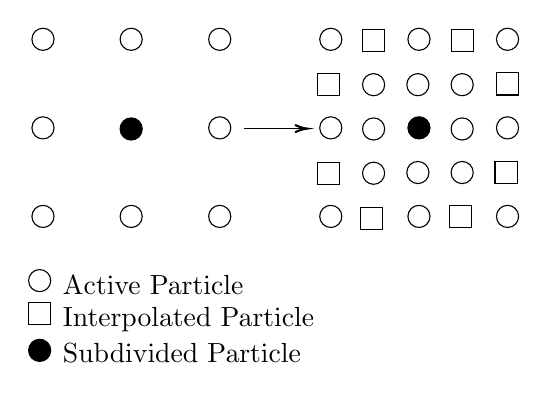
\begin{tikzpicture}[x=0.4pt,y=0.4pt,yscale=-1,xscale=1]
%uncomment if require: \path (0,425); %set diagram left start at 0, and has height of 425

%Shape: Circle [id:dp28714526119034034] 
\draw   (30.33,30.33) .. controls (30.33,24.81) and (34.81,20.33) .. (40.33,20.33) .. controls (45.86,20.33) and (50.33,24.81) .. (50.33,30.33) .. controls (50.33,35.86) and (45.86,40.33) .. (40.33,40.33) .. controls (34.81,40.33) and (30.33,35.86) .. (30.33,30.33) -- cycle ;
%Shape: Circle [id:dp9405531663649225] 
\draw   (110,30.33) .. controls (110,24.81) and (114.48,20.33) .. (120,20.33) .. controls (125.52,20.33) and (130,24.81) .. (130,30.33) .. controls (130,35.86) and (125.52,40.33) .. (120,40.33) .. controls (114.48,40.33) and (110,35.86) .. (110,30.33) -- cycle ;
%Shape: Circle [id:dp000891091912133879] 
\draw   (190,30.33) .. controls (190,24.81) and (194.48,20.33) .. (200,20.33) .. controls (205.52,20.33) and (210,24.81) .. (210,30.33) .. controls (210,35.86) and (205.52,40.33) .. (200,40.33) .. controls (194.48,40.33) and (190,35.86) .. (190,30.33) -- cycle ;
%Shape: Circle [id:dp2654804735412266] 
\draw   (30.33,110.33) .. controls (30.33,104.81) and (34.81,100.33) .. (40.33,100.33) .. controls (45.86,100.33) and (50.33,104.81) .. (50.33,110.33) .. controls (50.33,115.86) and (45.86,120.33) .. (40.33,120.33) .. controls (34.81,120.33) and (30.33,115.86) .. (30.33,110.33) -- cycle ;
%Shape: Circle [id:dp42179985152857613] 
\draw  [fill={rgb, 255:red, 0; green, 0; blue, 0 }  ,fill opacity=1 ] (110,111.33) .. controls (110,105.81) and (114.48,101.33) .. (120,101.33) .. controls (125.52,101.33) and (130,105.81) .. (130,111.33) .. controls (130,116.86) and (125.52,121.33) .. (120,121.33) .. controls (114.48,121.33) and (110,116.86) .. (110,111.33) -- cycle ;
%Shape: Circle [id:dp22630394337930826] 
\draw   (190,110.33) .. controls (190,104.81) and (194.48,100.33) .. (200,100.33) .. controls (205.52,100.33) and (210,104.81) .. (210,110.33) .. controls (210,115.86) and (205.52,120.33) .. (200,120.33) .. controls (194.48,120.33) and (190,115.86) .. (190,110.33) -- cycle ;
%Shape: Circle [id:dp6688016654819198] 
\draw   (30.33,190.33) .. controls (30.33,184.81) and (34.81,180.33) .. (40.33,180.33) .. controls (45.86,180.33) and (50.33,184.81) .. (50.33,190.33) .. controls (50.33,195.86) and (45.86,200.33) .. (40.33,200.33) .. controls (34.81,200.33) and (30.33,195.86) .. (30.33,190.33) -- cycle ;
%Shape: Circle [id:dp7311547975312614] 
\draw   (110,190.33) .. controls (110,184.81) and (114.48,180.33) .. (120,180.33) .. controls (125.52,180.33) and (130,184.81) .. (130,190.33) .. controls (130,195.86) and (125.52,200.33) .. (120,200.33) .. controls (114.48,200.33) and (110,195.86) .. (110,190.33) -- cycle ;
%Shape: Circle [id:dp9364435671025728] 
\draw   (190,190.33) .. controls (190,184.81) and (194.48,180.33) .. (200,180.33) .. controls (205.52,180.33) and (210,184.81) .. (210,190.33) .. controls (210,195.86) and (205.52,200.33) .. (200,200.33) .. controls (194.48,200.33) and (190,195.86) .. (190,190.33) -- cycle ;
%Shape: Circle [id:dp043369609467604264] 
\draw   (290.33,30.33) .. controls (290.33,24.81) and (294.81,20.33) .. (300.33,20.33) .. controls (305.86,20.33) and (310.33,24.81) .. (310.33,30.33) .. controls (310.33,35.86) and (305.86,40.33) .. (300.33,40.33) .. controls (294.81,40.33) and (290.33,35.86) .. (290.33,30.33) -- cycle ;
%Shape: Circle [id:dp43649566000313655] 
\draw   (370,30.33) .. controls (370,24.81) and (374.48,20.33) .. (380,20.33) .. controls (385.52,20.33) and (390,24.81) .. (390,30.33) .. controls (390,35.86) and (385.52,40.33) .. (380,40.33) .. controls (374.48,40.33) and (370,35.86) .. (370,30.33) -- cycle ;
%Shape: Circle [id:dp48984361894371486] 
\draw   (450,30.33) .. controls (450,24.81) and (454.48,20.33) .. (460,20.33) .. controls (465.52,20.33) and (470,24.81) .. (470,30.33) .. controls (470,35.86) and (465.52,40.33) .. (460,40.33) .. controls (454.48,40.33) and (450,35.86) .. (450,30.33) -- cycle ;
%Shape: Circle [id:dp21692313501267035] 
\draw   (290.33,110.33) .. controls (290.33,104.81) and (294.81,100.33) .. (300.33,100.33) .. controls (305.86,100.33) and (310.33,104.81) .. (310.33,110.33) .. controls (310.33,115.86) and (305.86,120.33) .. (300.33,120.33) .. controls (294.81,120.33) and (290.33,115.86) .. (290.33,110.33) -- cycle ;
%Shape: Circle [id:dp7820085896522643] 
\draw  [fill={rgb, 255:red, 0; green, 0; blue, 0 }  ,fill opacity=1 ] (370,110.33) .. controls (370,104.81) and (374.48,100.33) .. (380,100.33) .. controls (385.52,100.33) and (390,104.81) .. (390,110.33) .. controls (390,115.86) and (385.52,120.33) .. (380,120.33) .. controls (374.48,120.33) and (370,115.86) .. (370,110.33) -- cycle ;
%Shape: Circle [id:dp6243652554401846] 
\draw   (450,110.33) .. controls (450,104.81) and (454.48,100.33) .. (460,100.33) .. controls (465.52,100.33) and (470,104.81) .. (470,110.33) .. controls (470,115.86) and (465.52,120.33) .. (460,120.33) .. controls (454.48,120.33) and (450,115.86) .. (450,110.33) -- cycle ;
%Shape: Circle [id:dp17923992593808358] 
\draw   (290.33,190.33) .. controls (290.33,184.81) and (294.81,180.33) .. (300.33,180.33) .. controls (305.86,180.33) and (310.33,184.81) .. (310.33,190.33) .. controls (310.33,195.86) and (305.86,200.33) .. (300.33,200.33) .. controls (294.81,200.33) and (290.33,195.86) .. (290.33,190.33) -- cycle ;
%Shape: Circle [id:dp4427824930437838] 
\draw   (370,190.33) .. controls (370,184.81) and (374.48,180.33) .. (380,180.33) .. controls (385.52,180.33) and (390,184.81) .. (390,190.33) .. controls (390,195.86) and (385.52,200.33) .. (380,200.33) .. controls (374.48,200.33) and (370,195.86) .. (370,190.33) -- cycle ;
%Shape: Circle [id:dp6481215922758476] 
\draw   (450,190.33) .. controls (450,184.81) and (454.48,180.33) .. (460,180.33) .. controls (465.52,180.33) and (470,184.81) .. (470,190.33) .. controls (470,195.86) and (465.52,200.33) .. (460,200.33) .. controls (454.48,200.33) and (450,195.86) .. (450,190.33) -- cycle ;
%Shape: Circle [id:dp913831858550015] 
\draw   (369,71.33) .. controls (369,65.81) and (373.48,61.33) .. (379,61.33) .. controls (384.52,61.33) and (389,65.81) .. (389,71.33) .. controls (389,76.86) and (384.52,81.33) .. (379,81.33) .. controls (373.48,81.33) and (369,76.86) .. (369,71.33) -- cycle ;
%Shape: Circle [id:dp09461120708874005] 
\draw   (409,71.33) .. controls (409,65.81) and (413.48,61.33) .. (419,61.33) .. controls (424.52,61.33) and (429,65.81) .. (429,71.33) .. controls (429,76.86) and (424.52,81.33) .. (419,81.33) .. controls (413.48,81.33) and (409,76.86) .. (409,71.33) -- cycle ;
%Shape: Circle [id:dp25233682306463345] 
\draw   (409,111.33) .. controls (409,105.81) and (413.48,101.33) .. (419,101.33) .. controls (424.52,101.33) and (429,105.81) .. (429,111.33) .. controls (429,116.86) and (424.52,121.33) .. (419,121.33) .. controls (413.48,121.33) and (409,116.86) .. (409,111.33) -- cycle ;
%Shape: Circle [id:dp6505708685921722] 
\draw   (409,150.67) .. controls (409,145.14) and (413.48,140.67) .. (419,140.67) .. controls (424.52,140.67) and (429,145.14) .. (429,150.67) .. controls (429,156.19) and (424.52,160.67) .. (419,160.67) .. controls (413.48,160.67) and (409,156.19) .. (409,150.67) -- cycle ;
%Shape: Circle [id:dp5932001405334358] 
\draw   (369,150.67) .. controls (369,145.14) and (373.48,140.67) .. (379,140.67) .. controls (384.52,140.67) and (389,145.14) .. (389,150.67) .. controls (389,156.19) and (384.52,160.67) .. (379,160.67) .. controls (373.48,160.67) and (369,156.19) .. (369,150.67) -- cycle ;
%Shape: Circle [id:dp2796918706913195] 
\draw   (329,151.33) .. controls (329,145.81) and (333.48,141.33) .. (339,141.33) .. controls (344.52,141.33) and (349,145.81) .. (349,151.33) .. controls (349,156.86) and (344.52,161.33) .. (339,161.33) .. controls (333.48,161.33) and (329,156.86) .. (329,151.33) -- cycle ;
%Shape: Circle [id:dp17108368666663254] 
\draw   (329,111.33) .. controls (329,105.81) and (333.48,101.33) .. (339,101.33) .. controls (344.52,101.33) and (349,105.81) .. (349,111.33) .. controls (349,116.86) and (344.52,121.33) .. (339,121.33) .. controls (333.48,121.33) and (329,116.86) .. (329,111.33) -- cycle ;
%Shape: Circle [id:dp7721196012504834] 
\draw   (329,71.33) .. controls (329,65.81) and (333.48,61.33) .. (339,61.33) .. controls (344.52,61.33) and (349,65.81) .. (349,71.33) .. controls (349,76.86) and (344.52,81.33) .. (339,81.33) .. controls (333.48,81.33) and (329,76.86) .. (329,71.33) -- cycle ;
%Shape: Square [id:dp08655368923351381] 
\draw   (329,21.33) -- (349,21.33) -- (349,41.33) -- (329,41.33) -- cycle ;
%Shape: Square [id:dp6542243310151971] 
\draw   (288,61.33) -- (308,61.33) -- (308,81.33) -- (288,81.33) -- cycle ;
%Shape: Square [id:dp34824406004465147] 
\draw   (288,141.33) -- (308,141.33) -- (308,161.33) -- (288,161.33) -- cycle ;
%Shape: Square [id:dp46168142949503777] 
\draw   (327,182.33) -- (347,182.33) -- (347,202.33) -- (327,202.33) -- cycle ;
%Shape: Square [id:dp920301052069667] 
\draw   (407.67,180.67) -- (427.67,180.67) -- (427.67,200.67) -- (407.67,200.67) -- cycle ;
%Shape: Square [id:dp22091479839134276] 
\draw   (448.67,140.67) -- (468.67,140.67) -- (468.67,160.67) -- (448.67,160.67) -- cycle ;
%Shape: Square [id:dp552467747816834] 
\draw   (449.67,60.67) -- (469.67,60.67) -- (469.67,80.67) -- (449.67,80.67) -- cycle ;
%Shape: Square [id:dp6405559881104141] 
\draw   (409,21.33) -- (429,21.33) -- (429,41.33) -- (409,41.33) -- cycle ;
%Straight Lines [id:da7876300419244341] 
\draw    (222,111) -- (246,111) -- (277,111) ;
\draw [shift={(279,111)}, rotate = 180] [color={rgb, 255:red, 0; green, 0; blue, 0 }  ][line width=0.75]    (10.93,-3.29) .. controls (6.95,-1.4) and (3.31,-0.3) .. (0,0) .. controls (3.31,0.3) and (6.95,1.4) .. (10.93,3.29)   ;
%Shape: Circle [id:dp9364232594997858] 
\draw   (27.33,248.33) .. controls (27.33,242.81) and (31.81,238.33) .. (37.33,238.33) .. controls (42.86,238.33) and (47.33,242.81) .. (47.33,248.33) .. controls (47.33,253.86) and (42.86,258.33) .. (37.33,258.33) .. controls (31.81,258.33) and (27.33,253.86) .. (27.33,248.33) -- cycle ;
%Shape: Square [id:dp47304080161718076] 
\draw   (27,268.33) -- (47,268.33) -- (47,288.33) -- (27,288.33) -- cycle ;
%Shape: Circle [id:dp3927446610025478] 
\draw  [fill={rgb, 255:red, 0; green, 0; blue, 0 }  ,fill opacity=1 ] (27.33,311.33) .. controls (27.33,305.81) and (31.81,301.33) .. (37.33,301.33) .. controls (42.86,301.33) and (47.33,305.81) .. (47.33,311.33) .. controls (47.33,316.86) and (42.86,321.33) .. (37.33,321.33) .. controls (31.81,321.33) and (27.33,316.86) .. (27.33,311.33) -- cycle ;

% Text Node
\draw (56,241) node [anchor=north west][inner sep=0.75pt]   [align=left] {Active Particle};
% Text Node
\draw (56,270) node [anchor=north west][inner sep=0.75pt]   [align=left] {Interpolated Particle};
% Text Node
\draw (56,303) node [anchor=north west][inner sep=0.75pt]   [align=left] {Subdivided Particle};


\end{tikzpicture}
\caption{Subdividing around a point in the cloth mesh. In this case maximum subdivision $m=1$, and the new subdivided particles have $l=1$.}
\label{fig:subdiv}
\end{figure}
\subsection{Angle Based Subdivision Conditions}
The simpler of our 2 methods we use to determine subdivision points relies on the angles between cloth masses, and uses the same techniques outlined in \cite{hutchinson}. With this technique, we iterate over all indices of the cloth mesh. We then check if that index has either a spring above and below ($i\pm d$) or left and right ($j\pm d$). This $d$ is the same used when calculating particles connected via structural springs ($d=2^{m-l}$). For each of these pairs that exist, we then construct 2 vectors, each originating at our central $(i,j)$ point, and then extending to the adjacent 2 points. We then calculate the angle between these vectors, and if it is above a certain threshold, we subdivide around the central point. 
\subsection{Hanging Spring Subdivision Conditions}
While angle based subdivision provides us with a method to subdivide the mesh, it does not account for all scenarios we may wish to do so. For instance, consider the trivial cloth shown in Figure \ref{fig:hang}. If the top particles remain fixed, intuition would suggest that the center should be subdivided to allow the cloth to hang. Because there is no central point to create an angle, however, this mesh will never subdivide. 

\begin{figure}
\tikzset{every picture/.style={line width=0.75pt}} %set default line width to 0.75pt        

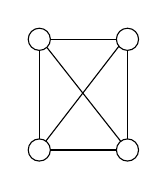
\begin{tikzpicture}[x=0.4pt,y=0.4pt,yscale=-1,xscale=1]
%uncomment if require: \path (0,300); %set diagram left start at 0, and has height of 300

%Shape: Circle [id:dp7708110690404341] 
\draw   (61.33,32.33) .. controls (61.33,26.81) and (65.81,22.33) .. (71.33,22.33) .. controls (76.86,22.33) and (81.33,26.81) .. (81.33,32.33) .. controls (81.33,37.86) and (76.86,42.33) .. (71.33,42.33) .. controls (65.81,42.33) and (61.33,37.86) .. (61.33,32.33) -- cycle ;
%Shape: Circle [id:dp7665280557032523] 
\draw   (141,32.33) .. controls (141,26.81) and (145.48,22.33) .. (151,22.33) .. controls (156.52,22.33) and (161,26.81) .. (161,32.33) .. controls (161,37.86) and (156.52,42.33) .. (151,42.33) .. controls (145.48,42.33) and (141,37.86) .. (141,32.33) -- cycle ;
%Shape: Circle [id:dp8143191905899676] 
\draw   (61.33,132.33) .. controls (61.33,126.81) and (65.81,122.33) .. (71.33,122.33) .. controls (76.86,122.33) and (81.33,126.81) .. (81.33,132.33) .. controls (81.33,137.86) and (76.86,142.33) .. (71.33,142.33) .. controls (65.81,142.33) and (61.33,137.86) .. (61.33,132.33) -- cycle ;
%Shape: Circle [id:dp055131028649787805] 
\draw   (141,132.33) .. controls (141,126.81) and (145.48,122.33) .. (151,122.33) .. controls (156.52,122.33) and (161,126.81) .. (161,132.33) .. controls (161,137.86) and (156.52,142.33) .. (151,142.33) .. controls (145.48,142.33) and (141,137.86) .. (141,132.33) -- cycle ;
%Straight Lines [id:da4031336052941048] 
\draw    (81.33,32.33) -- (141,32.33) ;
%Straight Lines [id:da8685025102332997] 
\draw    (151,122.33) -- (151,42.33) ;
%Straight Lines [id:da6758735308566833] 
\draw    (141,132.33) -- (81.33,132.33) ;
%Straight Lines [id:da8974623371735779] 
\draw    (71.33,42.33) -- (71.33,122.33) ;
%Straight Lines [id:da6410792423648672] 
\draw    (78.33,39.83) -- (144.67,124.17) ;
%Straight Lines [id:da5559775946796298] 
\draw    (143.33,38.5) -- (77.33,124.17) ;
\end{tikzpicture}
\caption{The simplest possible input cloth mesh. This mesh will never subdivide with angle based subdivision conditions, as it is not dense enough to measure any angles.}
\label{fig:hang}
\end{figure}

To combat this, we have introduced a new branch of subdivision conditions called "hanging springs". Similar to angle based subdivision, we begin by iterating over the cloth mesh and finding particles connected via structural springs. Instead of looking at both sides, however, we consider each connected particle one at a time. Let us refer to our input particle as $A$ and a structurally connected particle as $B$. We then imagine "hanging" our spring between $A$ and $B$, and using the midpoint along this path to calculate a new angle. With this new point, we can perform our initial angle based subdivision rules to determine if subdividing would allow the simulation to produce a hanging effect.

To solve for this hanging midpoint $M$, we first project $A$ and $B$'s position from $\mathbb{R}^3$ to $\mathbb{R}^2$. Since we are concerned with the cloth's ability to hang with gravity, we make sure that our projection allows for free gravitational movement. This is equivalent to projecting onto a plane with a normal orthogonal to the gravity vector, which for our simulation is along the y axis. To further simplify, we center our $\mathbb{R}^2$ projection such that $A$ is placed at $(0,0)$ . This gives us the projection from our $\mathbb{R}^3$ world space into projection space as:
\[
p(x,y,z) = (x-A_x, z-A_z)
\] 
We then further reduce the problem by approximating the path of the hanging spring as a parabola. While hanging objects naturally form catenaries rather than parabolas, the approximation is significantly simpler to compute and provides a similar midpoint. With this, we have reduced our hanging spring generation into finding a parabola that goes through both point $A$ and point $B$. When plugging these into a standard parabolic equation, we can see that any valid solution to this problem must take the form:
\[
f(x) = \alpha x^2+\left(\frac{B_y}{B_x}-\alpha B_x\right)x
\]
This, however, represents a set of infinitely many parabolas, as determined by the $\alpha$ constant. To solve for this, we ask the user for a new input: the hanging coefficient, $h$. With this coefficient, we add a new requirement to our hanging parabola: the arc length of the parabola between $A$ and $B$ must be a certain $l$, where
\[ l= \frac{h\cdot ||A_o-B_o||}{k}\]
In this equation, $k$ is the spring coefficient between $A$ and $B$, and $A_o, B_o$ are the original positions of the particles in our input mesh. If the particles did not exist in the input mesh, their original positions are linearly interpolated between the particles that were. This definition of length means that as we increase the stiffness of our springs, either through input parameters or subdivision, $A$ and $B$ must be forced closer together to trigger a subdivision. This intuitively aligns with the understanding that stiffer cloths will bend less.

To use this length $l$ to solve for $\alpha$, we must evaluate the arc length on our input and equate it to $l$. This can be calculated with the equation:
\[
l = \int \limits_{0}^{B_x}\sqrt{1+(2\alpha x+\frac{B_y}{B_x}-\alpha B_x)^2}\,dx
\]
This equation can be expanded to remove the integral, however, it ultimately remains analytically unsolvable. Therefore, we solve for $\alpha$ numerically in our simulation. Once we have $\alpha$ calculated, we simply solve for $f\left(\frac{B_x}{2}\right)$, and then project $\left(\frac{B_x}{2},f(\frac{B_x}{2})\right)$ into the $\mathbb{R}^3$ world space to perform our angle based decision.
\section{Results}
We tested out dynamic subdivision on a number of different input cloth meshes, and for each input tested 3 different categories of simulation:
\begin{itemize}
\item Simulation without any subdivision
\item Simulation with uniform subdivision across the mesh
\item Simulation with dynamic subdivision
\end{itemize}
The full table of these can be seen in Figure \ref{results}. When looking at completely unsubdivided meshes, a number of artifacts appear. This is particularly true on the pole and tablecloth simulations, where the lack of subdivision creates jagged artifacts as the corners of the mesh collapse. This is counteracted by the dynamic subdivision system, which much more closely mimics the fully subdivided mesh. 

This system, however, is not without its drawbacks, both in its results and its performance. We see that in these same situations, the dynamic subdivision remains unable to represent extra folds in the mesh that would appear with the pre-subdivided mesh. This is readily apparent in both our tablecloth and pole simulations, which create excess folds when simulated with higher fidelity. One way that this could be combated is to test for hanging spring subdivisions along the normal of a cloth quad in addition to along gravity, creating a sort of "popping spring" test. This, however, was out of the scope of testing for this paper.

While difficult to quantify, we do see a distinct speed disadvantage of the dynamic subdivision system whencompared to the complete lack of subdivision. To help combat this, we introduced an input parameter into the cloth input determining the frequency of subdivision checks. When the simulation checks for subdivision each frame, we see a slight but noticeable slowdown. This performance, however, remains orders of magnitude more performant in our tests than the pre-subdivided meshes.
\section{Conclusion \& Future Work}
Our dynamic subdivision system has a number of advantages, but also comes with a number of caveats. One of the primary caveats is due to an expansion of our cloth inputs when compared with those allowed in \cite{hutchinson}. In that original paper, it is presumed that there do not exist any angles in the original cloth mesh that would trigger a subdivision. Given this, when their simulation detects an angle based subdivision it can ``jump" back an animation step, perform subdivision, and continue on. Because our simulation allows for inputs that would trigger subdivisions in the first animation step, we cannot guarantee that there is a step to ``jump" back to. This has the result that any angle based subdivision system will trigger subdivisions up to the maximum subdivision depth. While this is not true for hanging spring decisions, it causes significant over subdivision with high maximum depths. One solution to this we experimented with was smoothing out subdivisions using the Loop subdivision scheme \cite{loop}, however we found that the smoothing on subdivision was jarring, and was not feasible for live use. One area of future work would be splitting subdivisions into 2 sections. If an angle based subdivision is triggered on the input mesh without simulation, then we would smooth the subdivision according to Loop's rules; however, if a subdivision occurred throughout the animation we would not perform any smoothing. This modifies the input mesh in such a way that we could guarantee future time steps could always ``jump" back to to a state not requiring subdivision. As such, we could use the time step fixes as described by \cite{hutchinson} for unlimited subdivision depth.

Beyond this 2 step subdivision there remain a number of areas for future work in this field. The first and most useful would be the implementation of dynamic subdivision in concert with a more modern cloth simulation technique. While the classic method we used \cite{provot} provides a functional cloth simulation, new techniques such as those discussed in \cite{largesteps} and \cite{collisions} provide substantially more physically accurate and potentially more performant cloth simulations. Applying the subdivision conditions discussed in this paper would be relatively simple; however, allowing for the simulation of arbitrary subdivisions would require more thorough research.

Another area of experimentation exists in a 2 phase approach to this dynamic subdivision. In the first phase, we would actively check for subdivisions as necessary, creating a smooth mesh when hanging. We could then pass this subdivided mesh as input into phase 2, which would then not actively check for more subdivisions. This second phase would be substantially faster than phase 1, but still remain smoothly subdivided. This 2 phase approach could be particularly useful in interactive environments where one would want to pre-compute a minimal mesh when resting that could then interact with ambient factors or user interaction faster than our current systems.
\section{Division of Labour}
While some of the work for this project was inherently collaborative, the project can approximately be broken down by person as the following:
\subsection*{Eleanor Olson}
\begin{itemize}
    \item Implemented the layered simulation according to the specifications of \cite{hutchinson}
    \item Implemented the subdivision of the underlying cloth mesh.
    \item Designed and implemented the rendering of a subdivided cloth mesh to quads.
    \item Designed and implemented the ideas surrounding hanging spring subdivisions.
    \item Wrote the slideshow presentation accompanying the paper.
    \item Wrote the Methods of Simulation, Results, and Conclusion sections of this paper.
\end{itemize}
\subsection*{Kana Rudnick}
\begin{itemize}
    \item Implemented iteration of the cloth mesh for subdivision decisions.
    \item Implemented Angle Based spring decisions.
    \item Determined base ideas around potential subdivision conditions.
    \item Assisted with debugging of various sections of the simulation.
    \item Wrote the Introduction and Related Work sections of this paper.
\end{itemize}
\section{Acknowledgments}
The groundwork for this simulation software was written by Professor Cutler for use in the homework of her Advanced Computer Graphics course, of which this paper is a product. This provided the basic parsing of object files, as well as rendering via both OpenGL and Metal. Additionally, this software provided us numerous tools for interactive with 3D objects and a robust vector library.

All of the code written for this project can be found on \href{https://github.com/eleanormally/dynamic-cloth}{GitHub} (\url{https://github.com/eleanormally/dynamic-cloth}). Our work is implemented in C++, and should run on all major operating systems, provided that OpenGL or Metal development frameworks are installed.
\setcitestyle{numbers}
\bibliographystyle{ACM-Reference-Format}
\bibliography{bib}
\begin{figure*}
\centering
\begin{tabularx}{\textwidth}{cccc}
\, &No Subdivision & Dynamic Subdivision & Uniform Subdivision \\
\text{Sheet} & \includegraphics[width=0.25\textwidth]{original_no_sub.png} &
\includegraphics[width=0.25\textwidth]{original.png} &
\includegraphics[width=0.25\textwidth]{original_pre_sub.png} \\
\text{Tablecloth} & \includegraphics[width=0.25\textwidth]{tablecloth_no_sub.png} &
\includegraphics[width=0.25\textwidth]{tablecloth.png} &
\includegraphics[width=0.25\textwidth]{tablecloth_pre_sub.png} \\
\text{Pole} & \includegraphics[width=0.25\textwidth]{pole_no_sub.png} &
\includegraphics[width=0.25\textwidth]{pole.png} &
\includegraphics[width=0.25\textwidth]{pole_pre_sub.png} \\
\end{tabularx}
\caption{An example of different input cloths with various categories of subdivision. Each dynamic subdivision cloth was limited to 1 layer of maximum subdivision, and uniform subdivision similarly adhered to this single subdivision layer.}
    \label{results}
\end{figure*}
\end{document}


